\documentclass[12pt, oneside]{article}
\usepackage[letterpaper, margin=1in]{geometry}
\usepackage[english]{babel}
\usepackage[utf8]{inputenc}
\usepackage{amsmath}
\usepackage{amsfonts}
\usepackage{amssymb}
\usepackage{tikz}
%\usepackage{tkz-fct}
\usepackage{pgfplots}
\pgfplotsset{width=10cm,compat=1.9}
\usepgfplotslibrary{statistics}
\usepackage{pgfplotstable}
%\usepackage{venndiagram}

\usepackage{fancyhdr}
\pagestyle{fancy}
\fancyhf{}
\rhead{\thepage \\Name: \hspace{1.5in}}
\lhead{BECA / Dr. Huson / 11.2 Algebra II\\* 23 April 2018 \\*\textbf{Do Now: Regression of bivariate data
}}

\renewcommand{\headrulewidth}{0pt}

\title{pgfplots template}
\author{Chris Huson}
\date{April 2018}

\begin{document}
%\maketitle
\subsubsection*{\\ \textnormal{The flash rate of fireflies depends on various factors, including temperature. As the temperature drops, the flash rate slows down.
}}

%\begin{enumerate}

%\item  Assume the given data

%\subsubsection*{Table of timing data}
%\item 
Firefly field data (simulated) where $T$ is the temperature and $f(T)$ is the number of seconds between flashes. \\[10pt]
\begin{tabular}{|c|r|r|r|r|r|}
\hline 
$T$ & 54 & 60 & 64 & 70 & 75 \\ [3pt]
\hline 
$f(T)$ & 5 & 8 & 10 & 11 & 13  \\  [3pt]
\hline 
\end{tabular}
\begin{enumerate}
    \item Plot the data in the table on the grid below \\
    (one point is plotted for you)
    \item Calculate the averages of both the temperature and flash period data. \\[50pt]
    \item Enter the data in your calculator and write down the correlation coefficient, $r$. \\[20pt]
    \item Approximately what how many seconds between each flash would you expect at $68^\circ F$?
\end{enumerate}

\vspace{0.5in}
%\item 
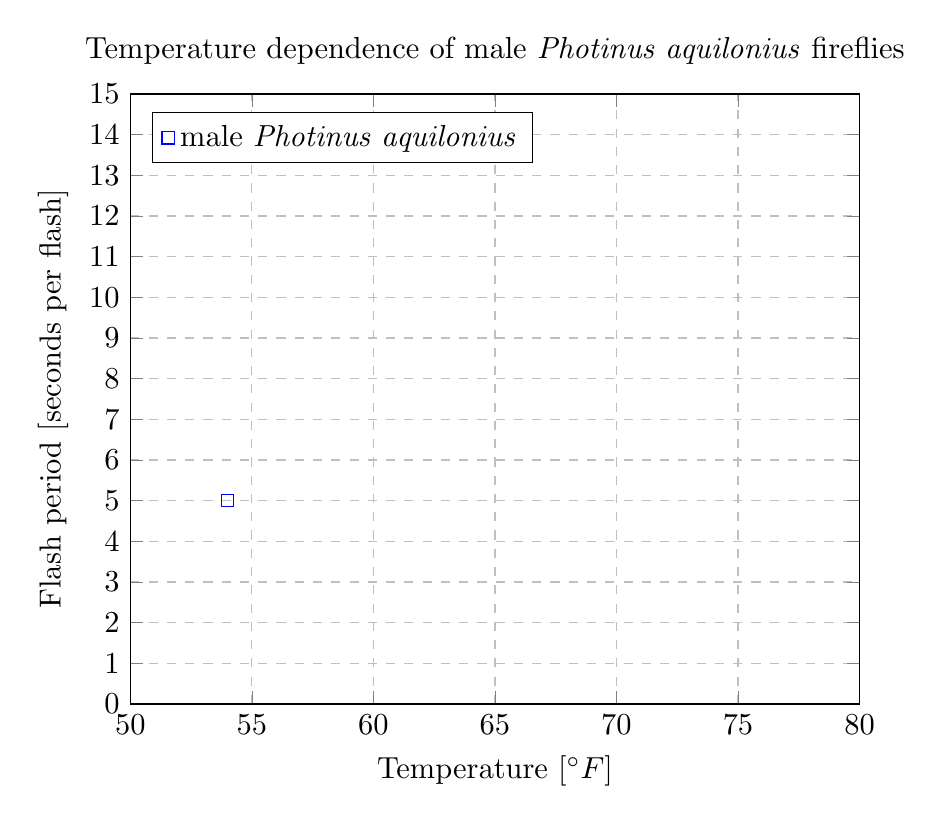
\begin{tikzpicture}[scale=1.1]
\begin{axis}[
    title={Temperature dependence of male \emph{Photinus aquilonius} fireflies},
    xlabel={Temperature [$^{\circ}F$]},
    ylabel={Flash period [seconds per flash]},
    xmin=50, xmax=80,
    ymin=0, ymax=15,
    xtick={50,55,60,65,70,75,80},
    ytick={0,1,2,3,4,5,6,7,8,9,10,11,12,13,14,15},
    legend pos=north west,
    xmajorgrids=true,
    ymajorgrids=true,
    grid style=dashed,
]
\addplot[only marks,
    color=blue,
    mark=square,
    ]
    coordinates {
    (54,5)%(60,8)(64,10)(70,11)(75,13)
    };
    \legend{male \emph{Photinus aquilonius}}
\end{axis}
\end{tikzpicture}


%\end{enumerate}
\end{document}